\documentclass{article} % For LaTeX2e
% We will use NIPS submission format
\usepackage{nips13submit_e,times}
% for hyperlinks
\usepackage{hyperref}
\usepackage{url}
% For figures
\usepackage{graphicx} 
\usepackage{subfigure} 
% math packages
\usepackage{amsmath}
\usepackage{amsfonts}
\usepackage{amsopn}
\usepackage{ifthen}
\usepackage{natbib}

\title{Project-I by Group AUCKLAND}

\author{
Marco Goretti \And Pascal Lau \And Pierre Gabioud \\
\texttt{} \\
}


\nipsfinalcopy 


\begin{document}

\maketitle

\begin{abstract}
In this report, we summarize our findings for the project 1. We run different experiments to improve our results and strive to obtain an ideal prediction for the given test data for regression and classification.

\end{abstract}

\section{Regression}
\subsection{Data Description}
Our train-data consists of output variable $\mathbf{y_{train}}$ and input variables $\mathbf{X_{train}}$ while our test-data consists of an input variable $\mathbf{X_{test}}$. We have $N=1400$ data examples. Each input vector $\mathbf{x}_n$ is of dimensionality $D$ = 48. Out of these 48 variables, 35 are real valued, 13 are categorical with 3 categories, 2 are categorical with 4 categories and finally 2 of them are binary.

We also have a set of $N=600$ test examples test-data $\mathbf{X_{test}}$ where we do not observe the related ouput $\mathbf{y}$. Our goal is to produce predictions for these test examples, as well as an approximation of the test-error.

\subsection{Data visualization and cleaning}
We started by a basic data analysis of our input. Figure \ref{fig:boxplotX} shows the distribution of the 35 real-valued input variables. As we can see, they are not centered so we normalized them. Figure \ref{fig:histY} shows the histogram of the output variable $\mathbf{y}$. We see that the distribution is separated in two groups, with one major group and another smaller group of higher values.
The correlation between the output and input variables is shown in Figure \ref{fig:correlations}. Again, we can see a clear separation of the results in two groups of values. Moreover, we notice a lack of direct correlation between most of the inputs and the output $\mathbf{y}$. We will later try to apply transformations to see if we can improve this point.

Another thing we observed is the correlation between inputs in  $\mathbf{X_{train}}$ , shown in Figure \ref{fig:correlationsX}. We can see a non-negligible correlation between a few of them, for example between input 28 and 30 with a correlation of 0.8. However they are in general weakly correlated which is a positive aspect for our analysis.


Finally, we checked the rank of the input matrix $\mathbf{X_{train}}$. It turned out that the rank is equal to the number of columns of the matrix so $\mathbf{X_{train}}$ is full-rank.

\begin{figure}[!t]
\center
\subfigure[Boxplot of real-valued $\mathbf{X}$. Data is not centered so we normalized it.]{\includegraphics[width=2.5in]{figures/boxplotX.pdf} \label{fig:boxplotX}}
\hfill
\subfigure[Histogram of $\mathbf{y}$. We see a gaussian distribution of some of the values and another group of values with another distribution (maybe chi-squared) ]{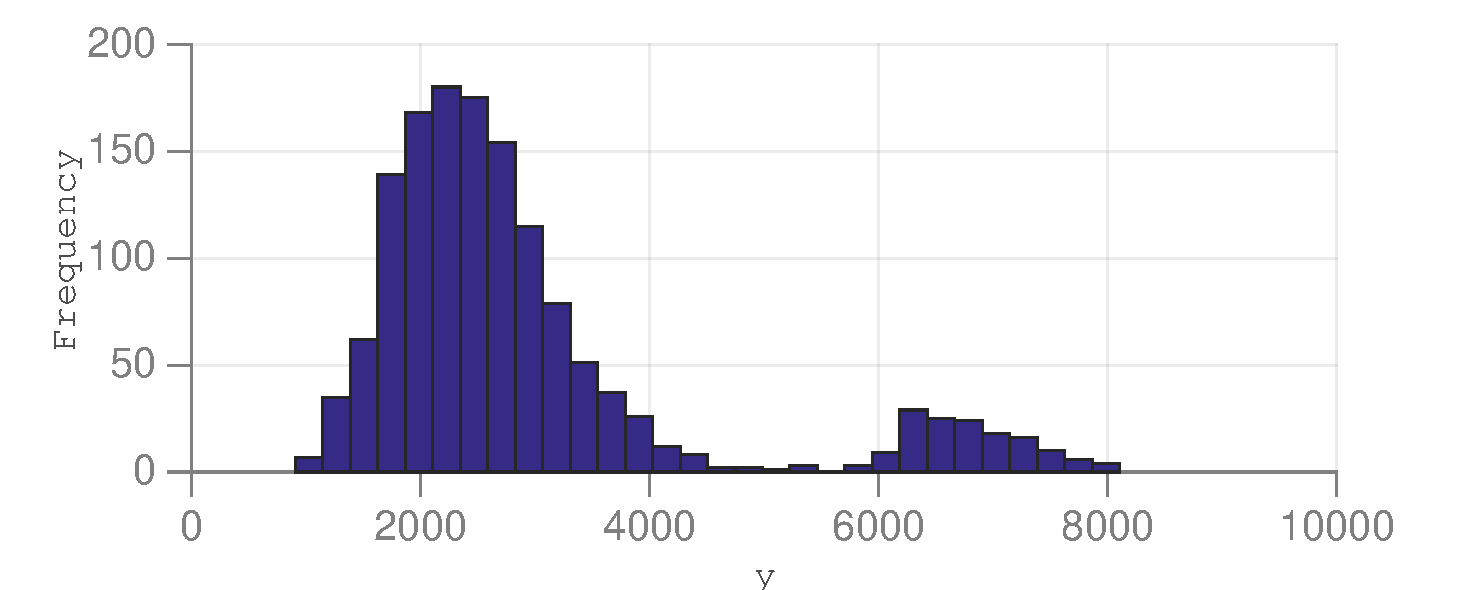
\includegraphics[width=2.5in]{figures/histY.pdf} \label{fig:histY}}
\caption{Data Analysis}
\end{figure}

\begin{figure}[!h]
\center

\subfigure[Correlations between each input in $\mathbf{X_train}$ and output $\mathbf{y}$]{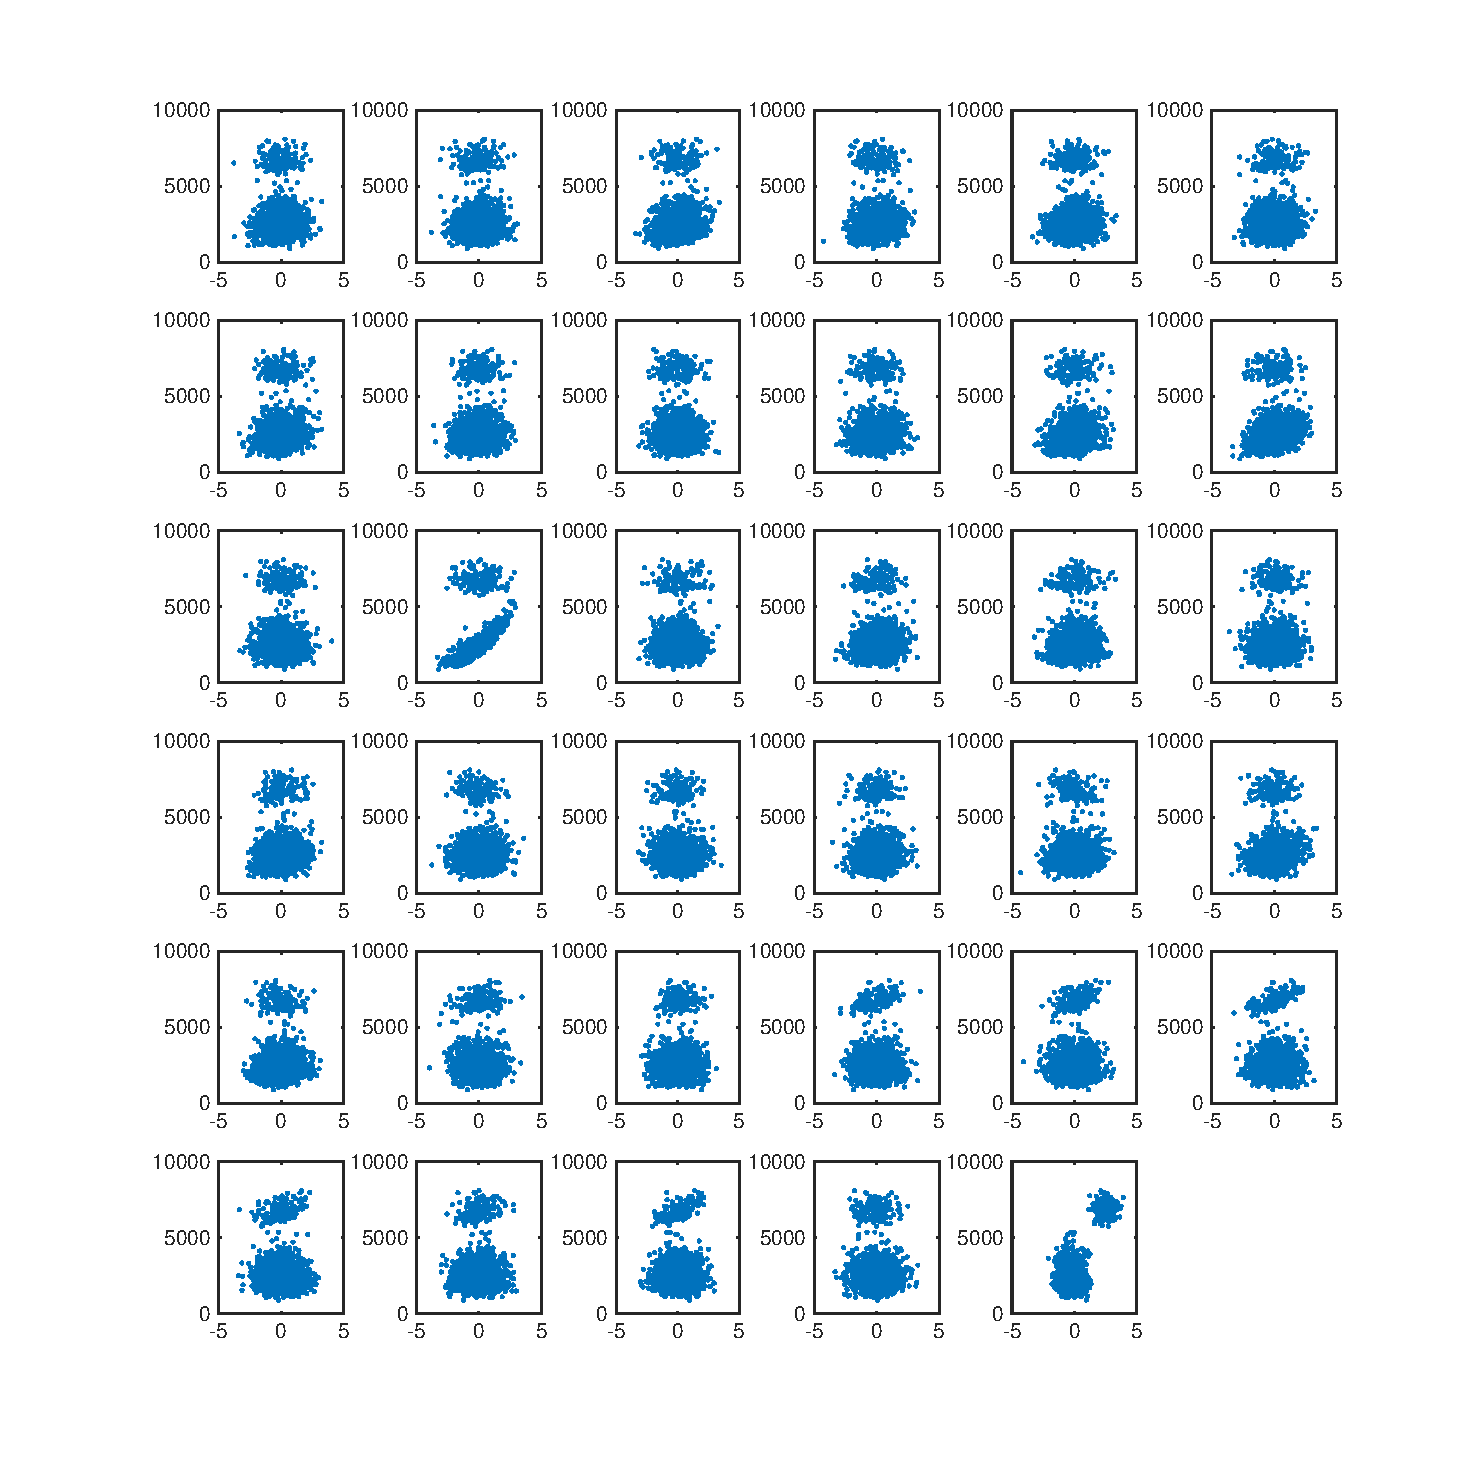
\includegraphics[width=2.5in]{figures/correlations.pdf} \label{fig:correlations}}
\hfill
\subfigure[Correlations between inputs in $\mathbf{X_train}$]{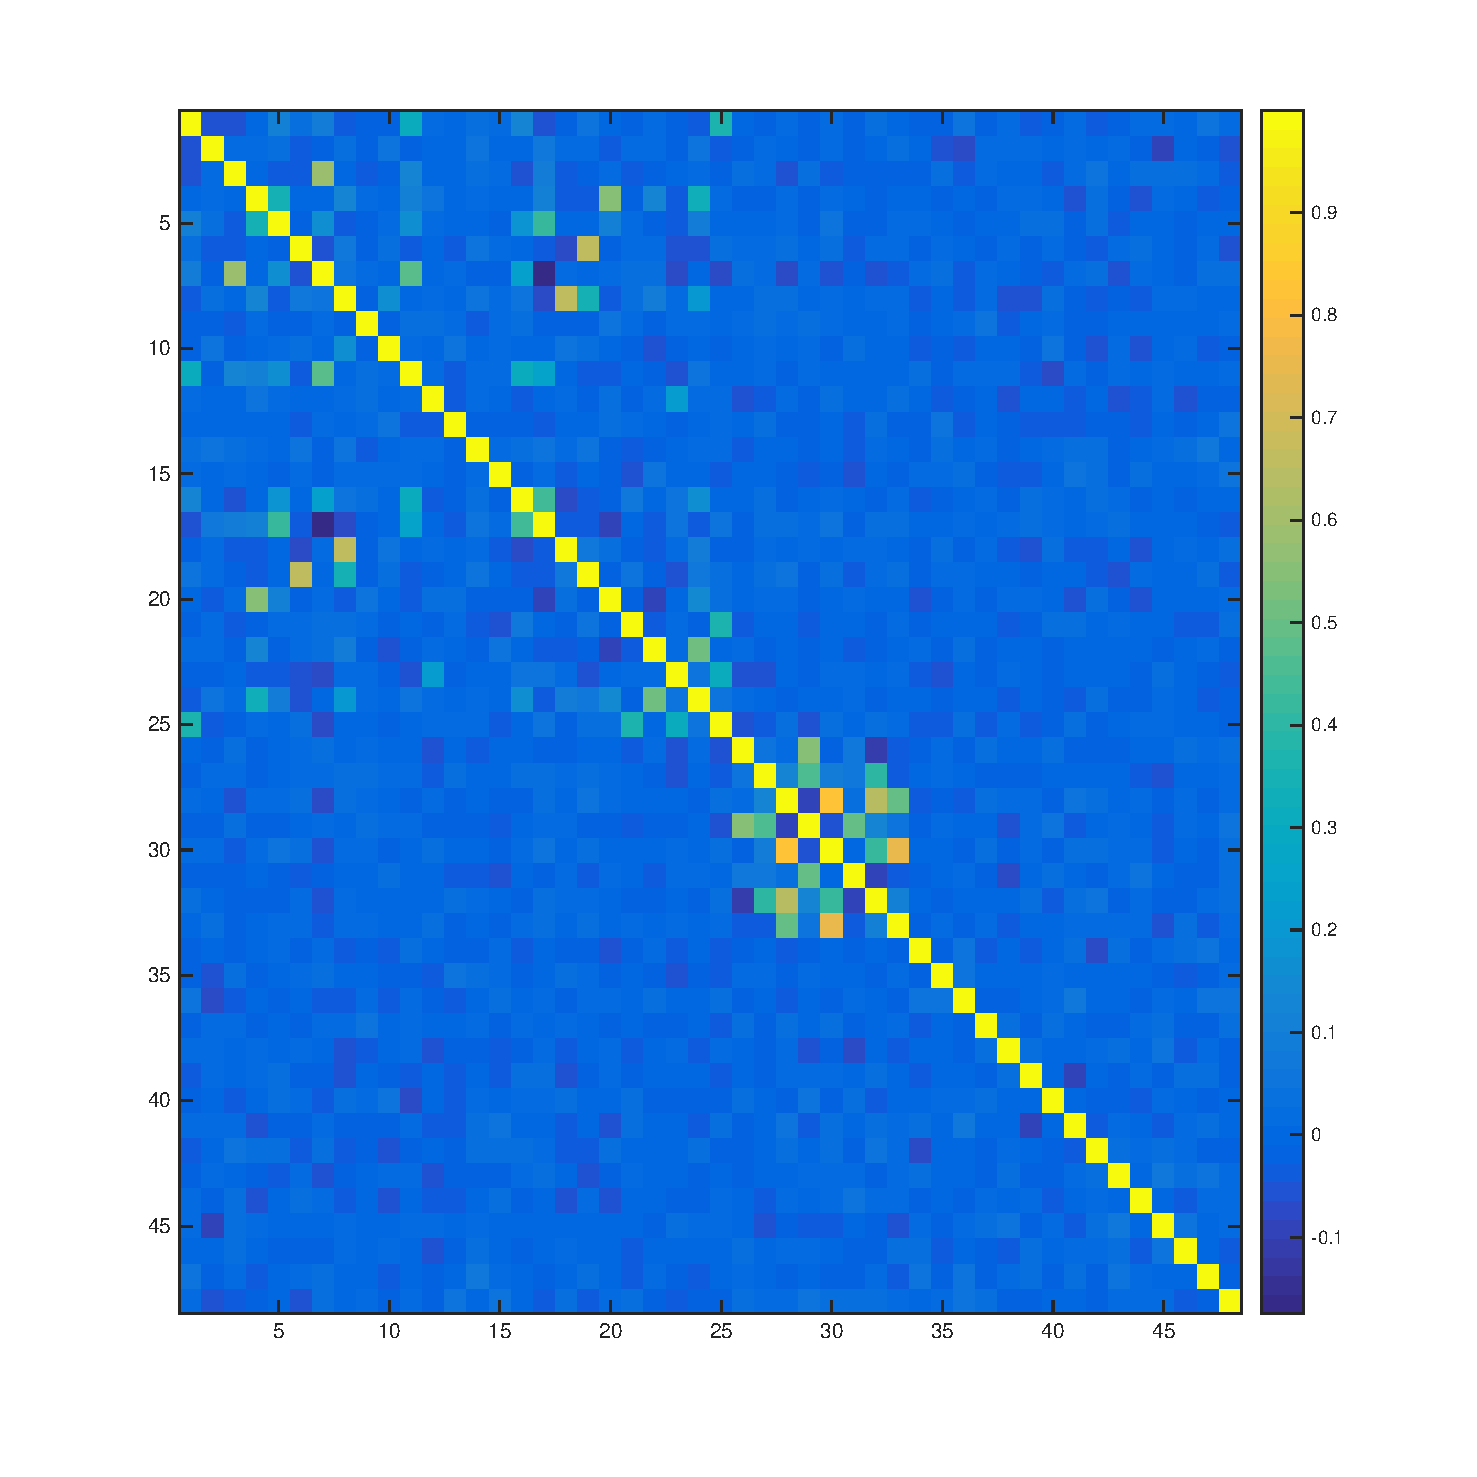
\includegraphics[width=2.5in]{figures/correlationsX.pdf} \label{fig:correlationsX}}
\caption{Correlations}
\end{figure}



\subsection{Linear regression}
We tried the different methods we implemented. Using ridge regression is not relevant in our case since we observed that our matrix is full-rank. To ensure our hypothesis is correct, we used ridge regression anyway and the results, as expected, confirmed our observation. We therefore used least squares to compute our vector beta. We implemented a K-fold test with $\frac{3}{10}$ of our data as test data and the rest as train data. By doing so, we have a proportion of test and train data corresponding to the dataset given where we had 1400 data in the training set and 600 given as test. 


\subsubsection{Unsuccessful experiments}

The first thing we tried was testing the interaction effects among the input data. That is, we multiplied $\mathbf{x_{i}}$ with $\mathbf{x_{j}}$ for all distinct $\mathbf{i}$ and $\mathbf{j}$. Then we sorted the results according to the correlation they had with $\mathbf{y}$. With all the interactions between all inputs and their respective correlation with $\mathbf{y}$, we were able to add them to our original feature set and see whether they improved our test results or not. We tried to add the \textit{n} best interactions but the results did not show any improvement. We think that this is because the explanatory variables we were adding were highly autocorrelated.

After that, we tried to add the less autocorrelated variables to our set of features to see if we could improve the test. The results were not satisfying either and the test error of our K-fold test was not improving. The reason is because they are also weakly correlated to $\mathbf{y}$. 

\subsubsubsection{Applying transformation}

We tried to apply, at random, different kind of transformations to our data to get a better grip of the data we are dealing with. Most of them however did not significantly reduce the error so we did not include the results in the report. We also tried features such as $X_{i}^{X_{j}}$ but the improvement was minimal with an increase in complexity.

\subsubsubsection{Removing useless features}

We tried to remove, one by one, every $\mathbf{x_{i}}$ $\forall$i to decrease the dimensionality but this increased the test error. We expected some of those to be overfitting the data because of their low correlation with y (few explication of y added) but we were wrong and they are all useful.


We tried to remove, one at the time, every $\mathbf{x_{i}}$ $\forall$i to decrease the error. In contrary to what we wanted, the error increased instead. Indeed, we thought that the low correlation between $\mathbf{x_{i}}$ and $\mathbf{y}$ would allow us to remove some of the $\mathbf{x_{i}}$. This experiment showed that we were wrong and low correlation between input and output does not imply useless features. 

\begin{figure}[!h]
\center

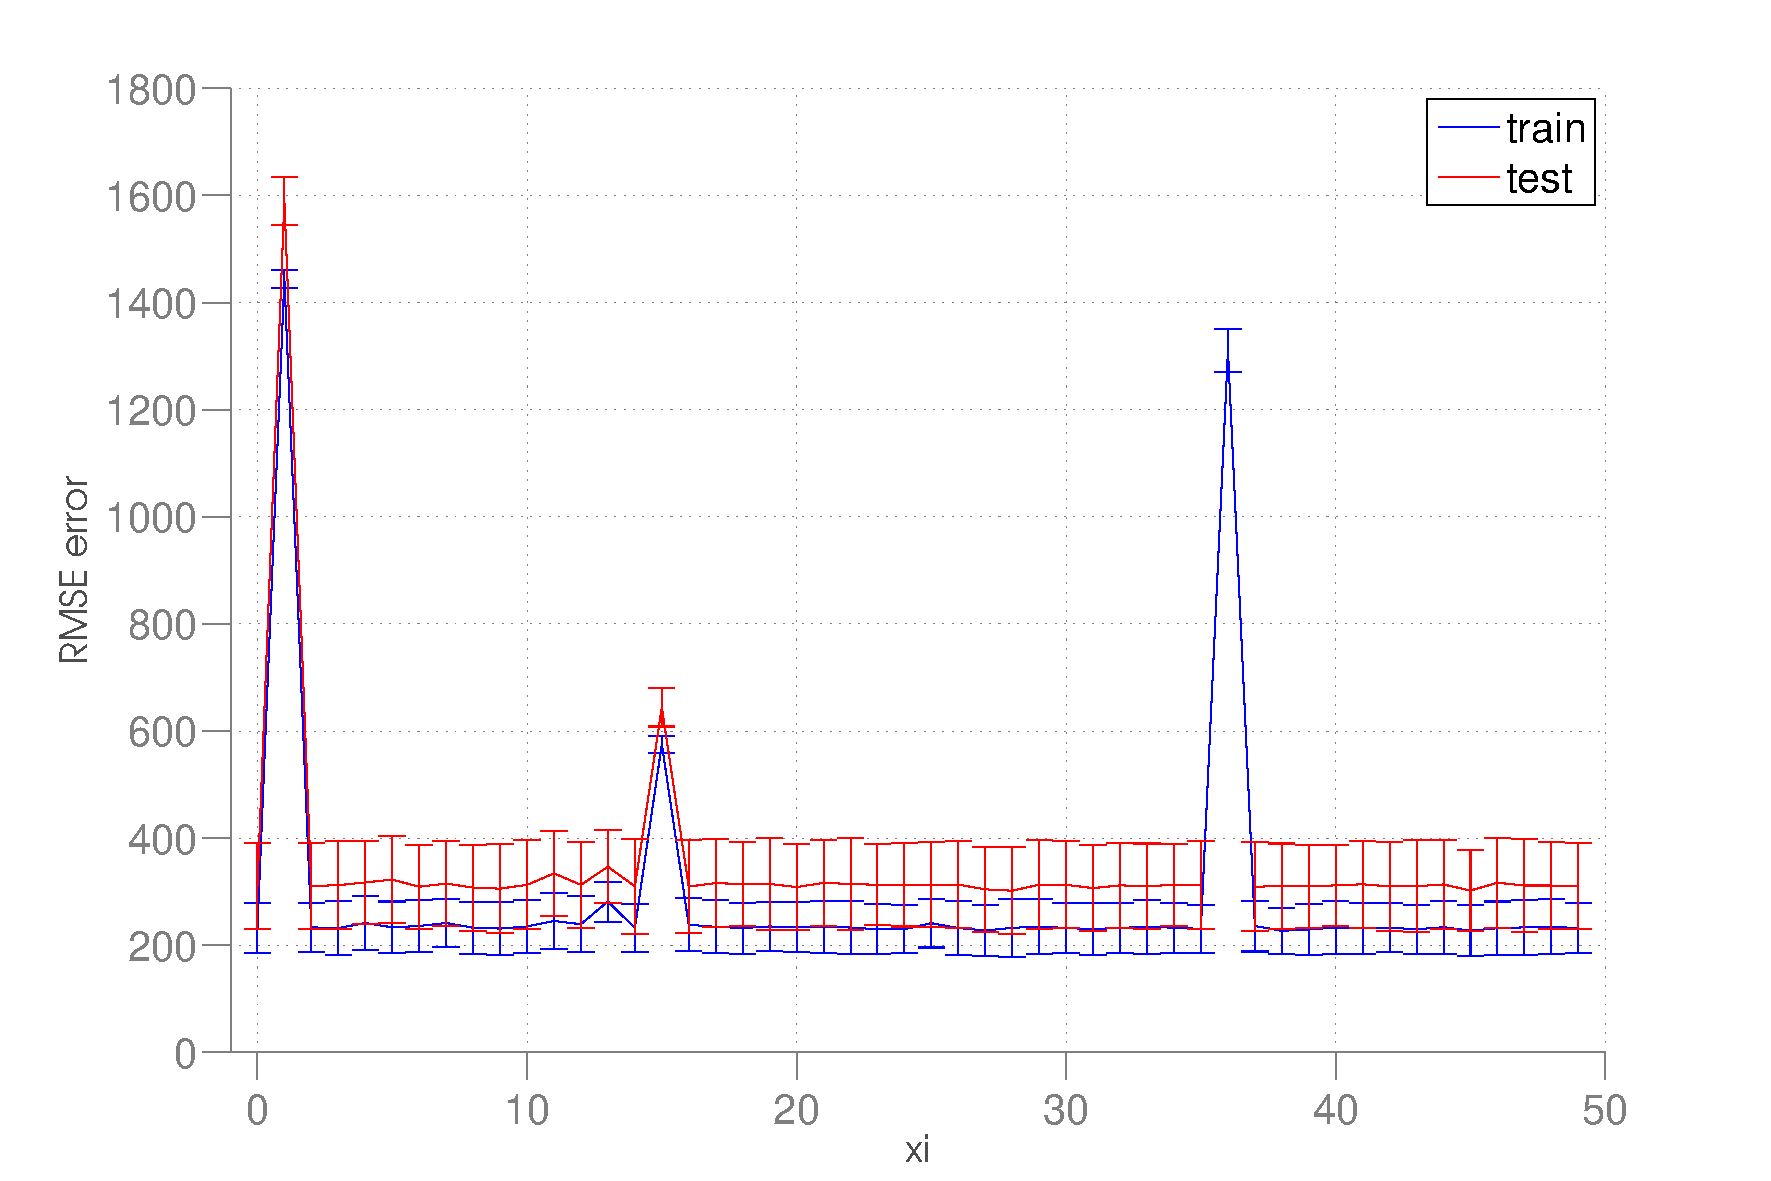
\includegraphics[width=2.5in]{figures/dimRed.pdf} 
\label{fig:dimRed}

\caption{Effect on error when removing  $\mathbf{x_{i}}$}
\end{figure}


\subsubsection{Successful experiments}
\subsubsubsection{Separating the dataset}

The results using our different techniques were not satisfying so we explored an alternative: separate the data into two sets. As we can see in Figure \ref{fig:correlations} and \ref{fig:histY}, two groups of values are clearly visible for every input. In order to find where to split the data, we determine the test and train errors using the same ratio of $\frac{3}{10}$ than in our k-fold. We can see in Figure \ref{fig:seperation} that a separation at around 5100 gives a minimized error for train and test. Then, we found by iteratively testing different values of $\alpha$ that the ideal value for our logistic regression is at around $\alpha$ $\approx$ 1.3, as shown on Figure \ref{fig:alphaRegression}.

\begin{figure}[!h]
\center

\subfigure[Train and test errors to find the ideal separation ]{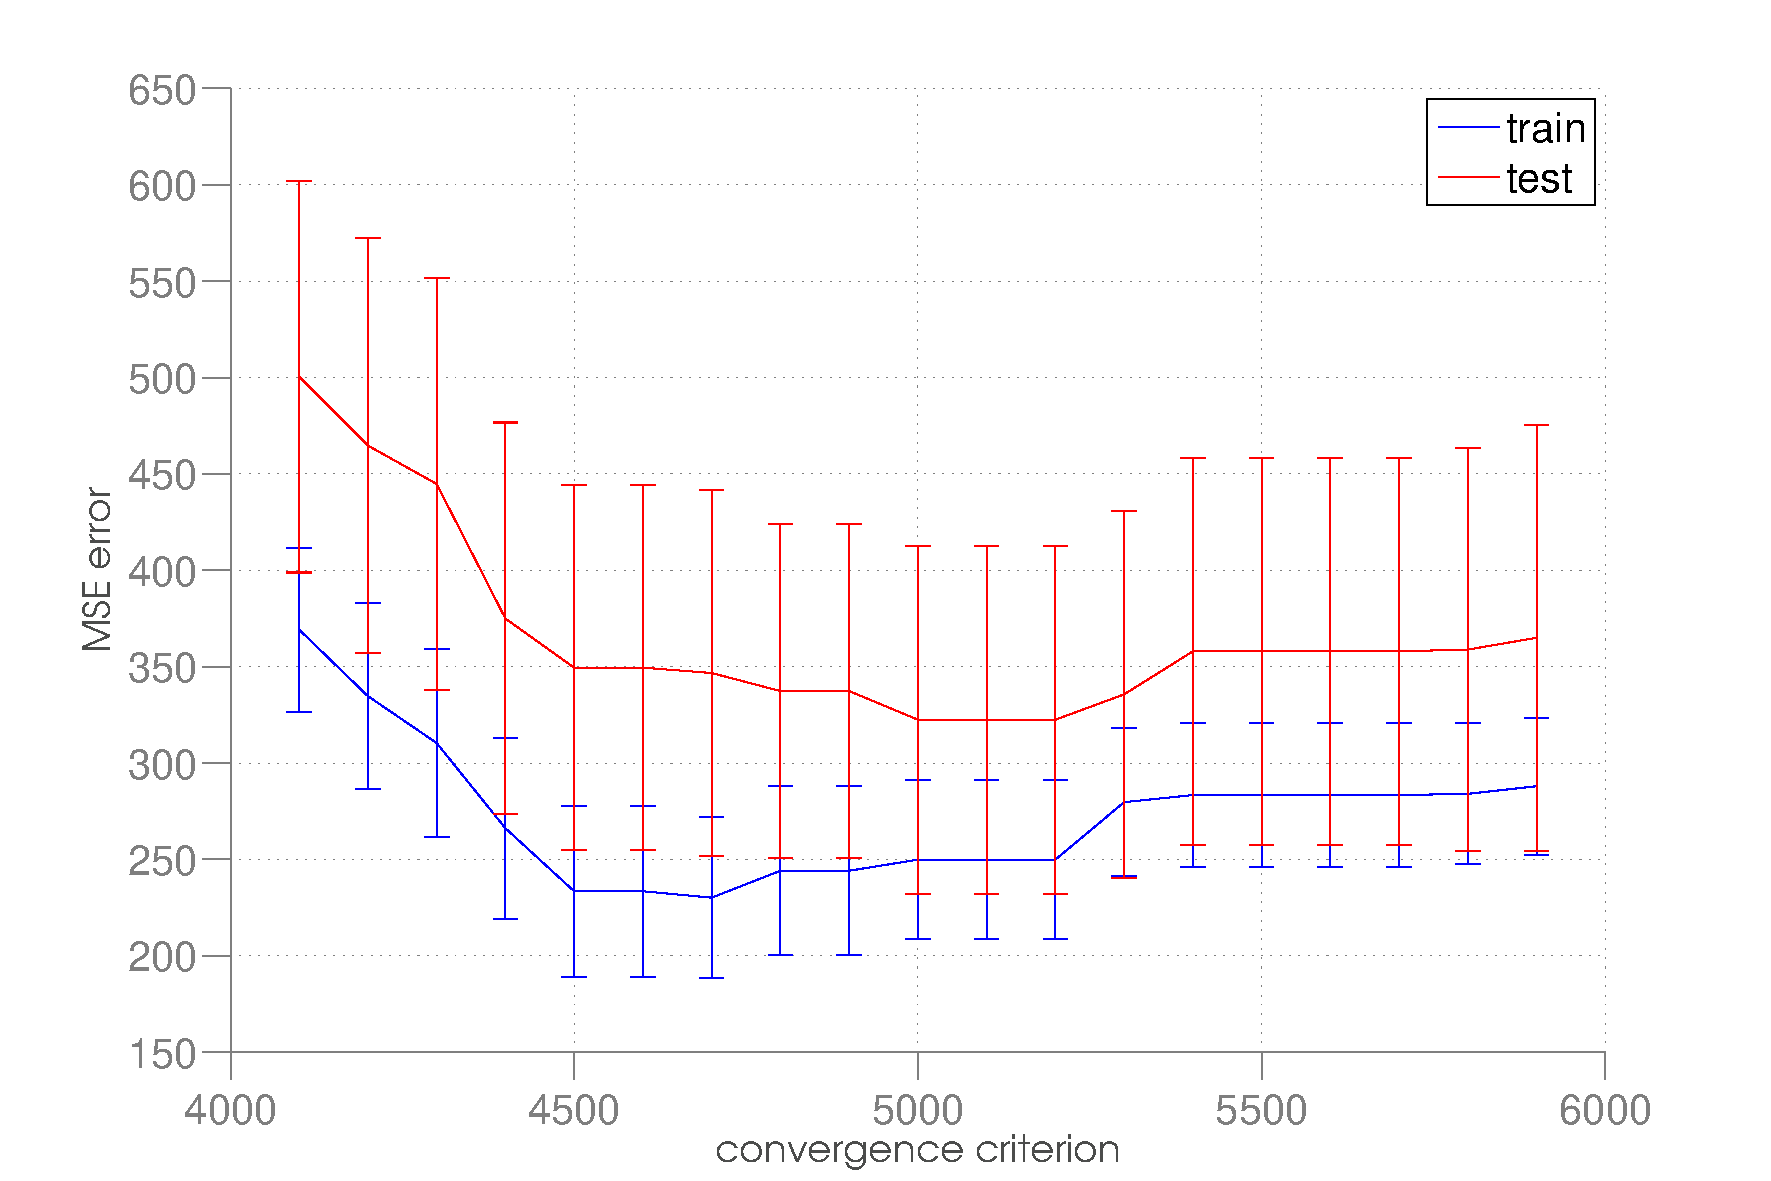
\includegraphics[width=2.5in]{figures/classificationWithRegression.pdf} \label{fig:seperation}}
\hfill
\subfigure[Alpha vs Mean Square Error]{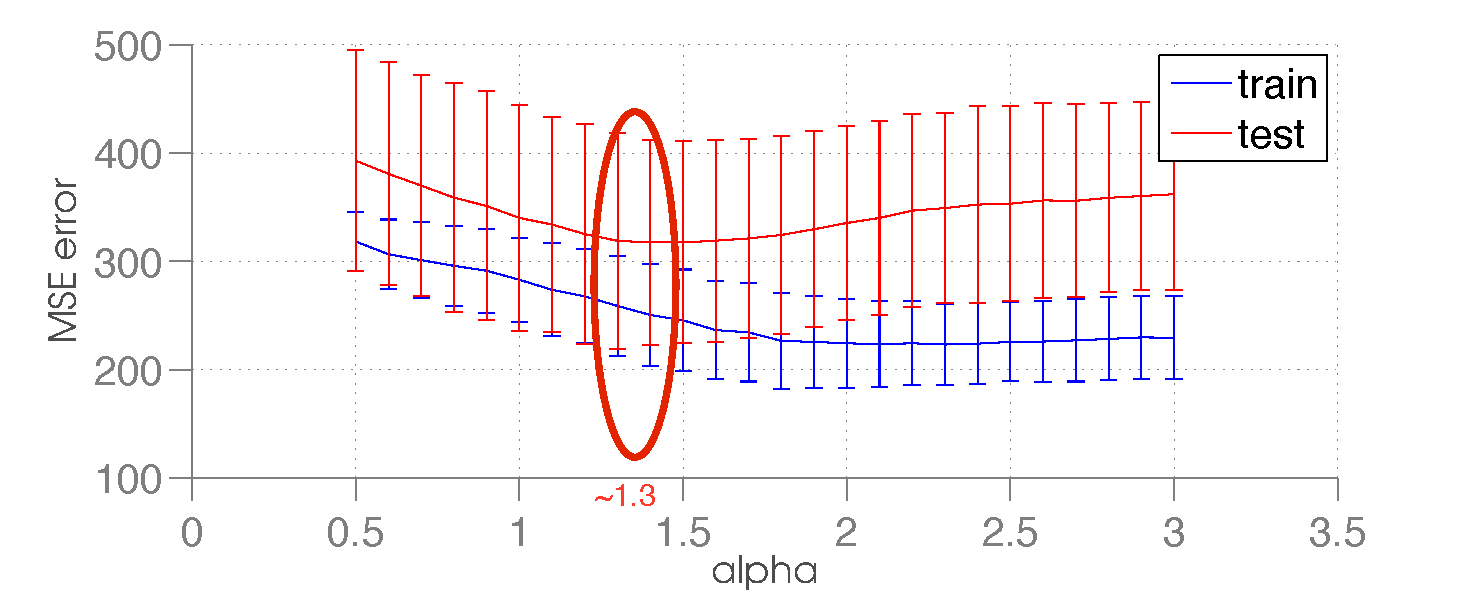
\includegraphics[width=2.5in]{figures/alphaRegression.pdf} \label{fig:alphaRegression}}
\caption{Evolution of MSE}
\end{figure}

\subsubsubsection{Applying transformations and interaction effects}
The next step of our analysis consists in finding out if any interaction effect $\mathbf{x_{i} \cdot x_{j}}$ can improve our test error. We test the effect of all the possibilities of interaction on the error and include the ones reducing the error the most. Figure \ref{fig:interactionReg} shows the error before adding the best interaction effects and Figure \ref{fig:interactionRegAfter} shows the error after adding them. We see an improvement.


\begin{figure}[!h]
\center
\subfigure[Train and test errors when adding interaction feature $\mathbf{x_{i} \cdot x_{j}}$ ]{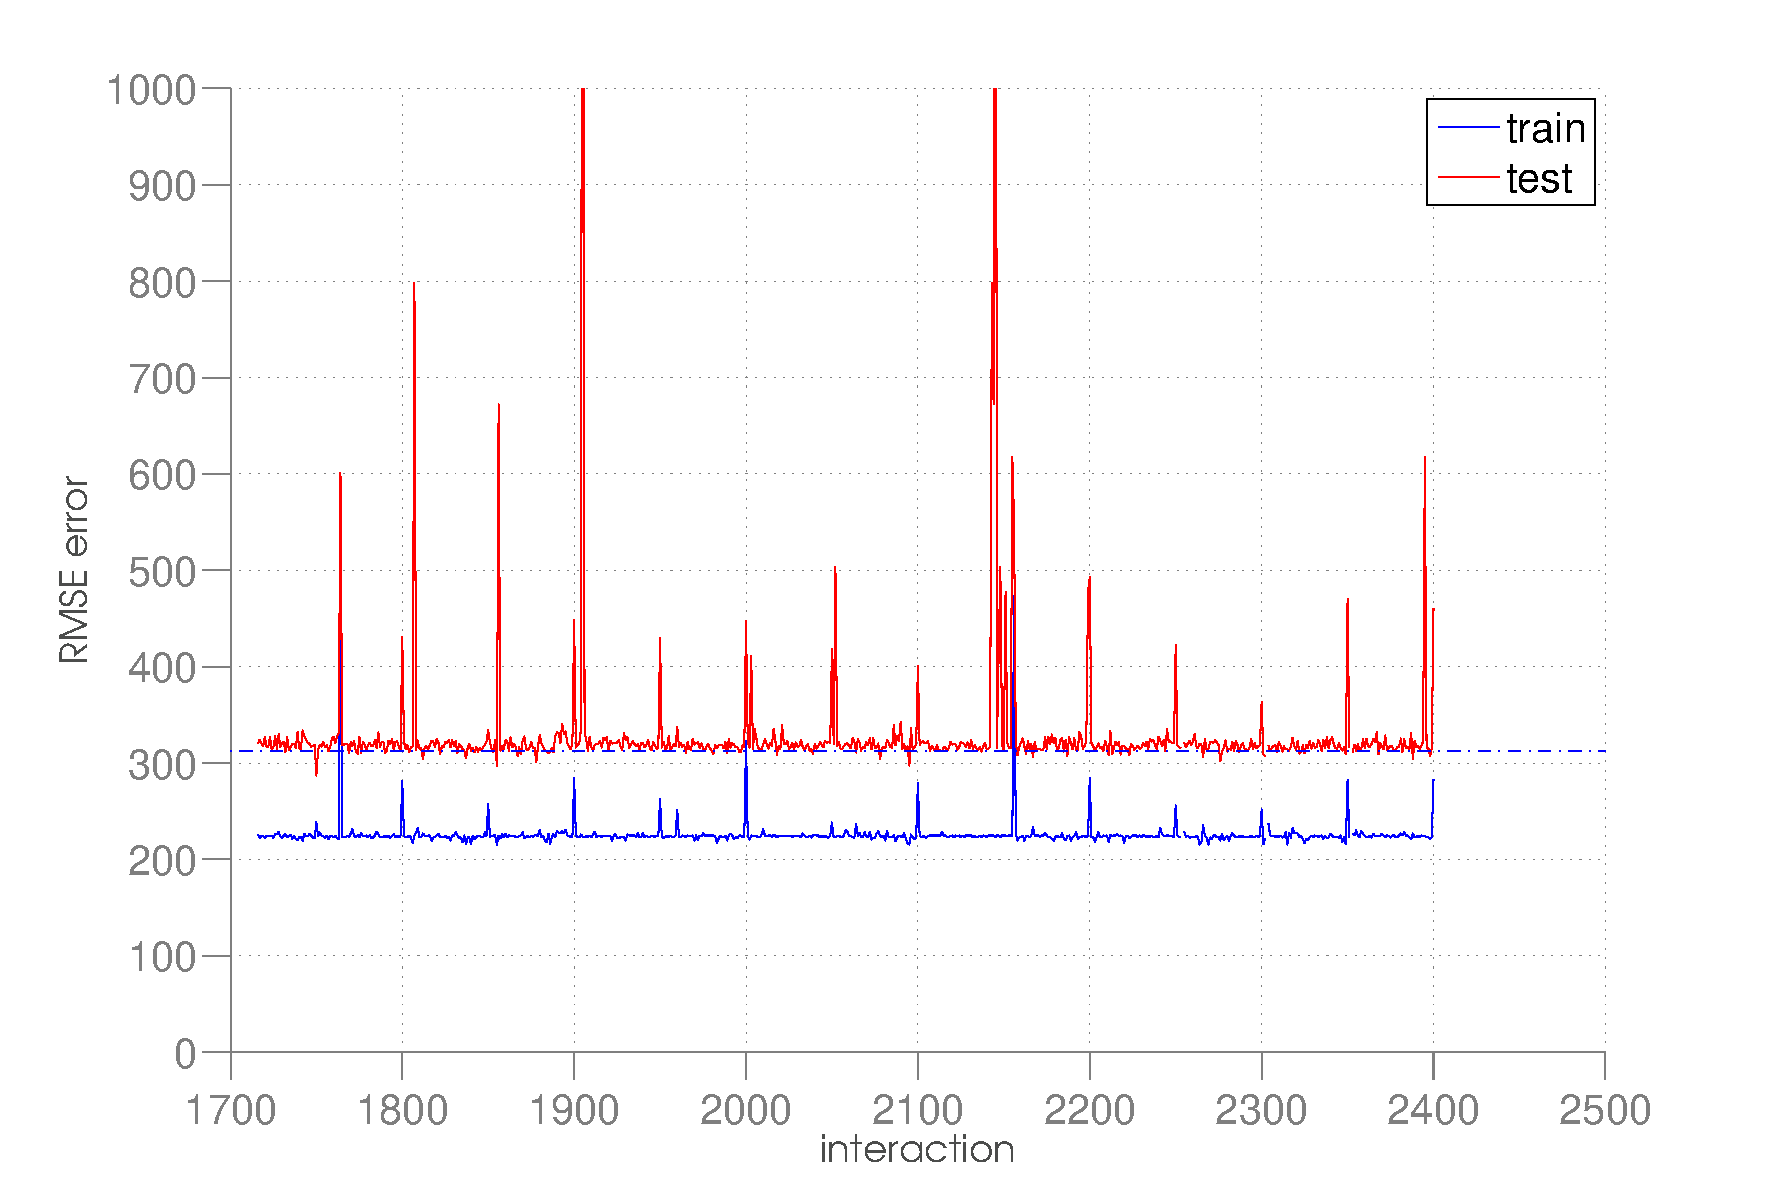
\includegraphics[width=2.5in]{figures/interactionReg.pdf}\label{fig:interactionReg}}
\hfill
\subfigure[Train and test errors after adding the best interaction features]{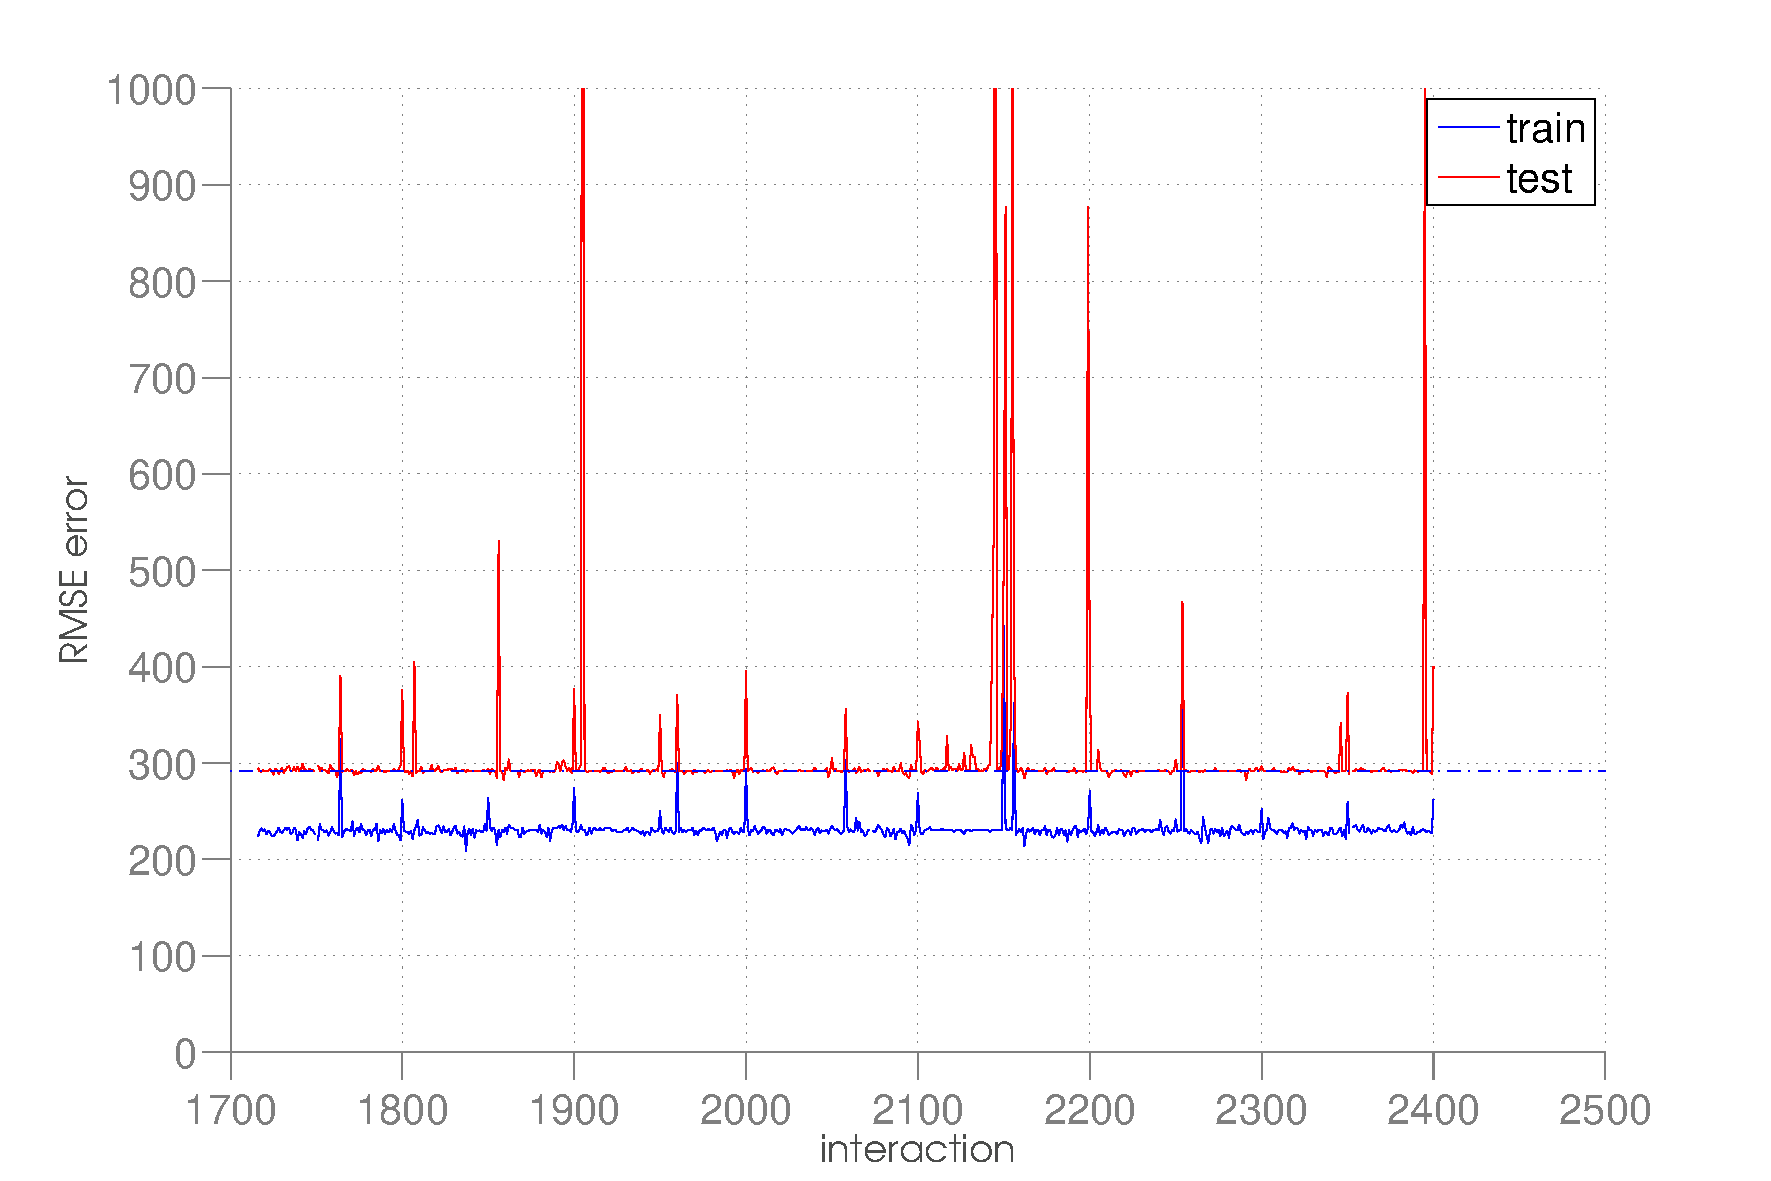
\includegraphics[width=2.5in]{figures/interactionRegAfter.pdf}\label{fig:interactionRegAfter}}
\caption{Effect on error using interactions  $\mathbf{x_{i} \cdot x_{j}}$ }
\end{figure}


\section{Classification}

In this section we explore the classification dataset. 
\subsection{Data Description}
Our train-data consists of binary output variable $\mathbf{y_{train}}$ and input variables $\mathbf{X_{train}}$. Our test-data consists of an input variable $\mathbf{X_{test}}$. Both train and test data have $N=1500$ observations. Each input vector $\mathbf{x}_n$ is of dimensionality $D$ = 22. Out of these 22 variables, 4 take integer values while the rest are real valued.

Once again, we do not have the related output $\mathbf{y}$ for our test-data $\mathbf{X_{test}}$. Our goal is to predict as accurately as possible the value of $\mathbf{y_{test}}$.

\subsection{Logistic Regression}
We first run logistic regression on our raw data in order to see how the following errors evolve with alpha: the \textit{Root-Mean-Square Error}, the \textit{0-1 Loss} and the \textit{log Loss}. We also tried to run the penalized logistic regression but we quickly realized that the results were not improved regardless of the value chosen for lambda. This result was expected since we did not encounter any computing issue when dealing with the matrix $\mathbf{X_{train}}$ in MATLAB. The results of the errors obtained with logistic regression are displayed in Figure \ref{fig:errors}. We see that all them evolve in the same way when alpha increases. Given this fact, we decided to focus on improving our RMSE, knowing that the other errors will decrease accordingly. We found an ideal value for alpha at $\alpha$ $\approx$ 1. We will use this value as reference in the next steps of our analysis. With this setting, we can see our first results for the \textit{0-1 Loss} at about 15\%, about 32\% for the RMSE and 37\% for the log-loss. We try to improve these results with different techniques described below.

\subsubsection{Dimension reduction}
We first try to check whether one or more features in $\mathbf{X_{train}}$ might be useless for our logistic regression. Figure \ref{fig:dimRefLR} shows how the RMSE changes when we remove $\mathbf{x_{i}}$. As depicted by the figure, the RMSE increases a lot when some of the features are removed but it never seems to decrease for any removed feature. Thus, we concluded that deleting an input from the set of features is not useful for our results.

\clearpage
\subsubsection{Feature transformation and interaction}
The next thing we tried was analysing the effect of interaction features $\mathbf{x_{i} \cdot x_{j}}$ on the RMSE. We can see in Figure \ref{fig:interaction} that adding some interactions can be useful to improve our test error. We found the best interactions and added them to our feature set. The results are clearly visible on Figure \ref{fig:interaction3}: we improved our 0-1 loss for train and test data from 15\% to 10\% and our RMSE went from 0.32 to 0.27.


\begin{figure}[!htb]
\center
\subfigure[Evolution of errors with respect to alpha in logistic regression]{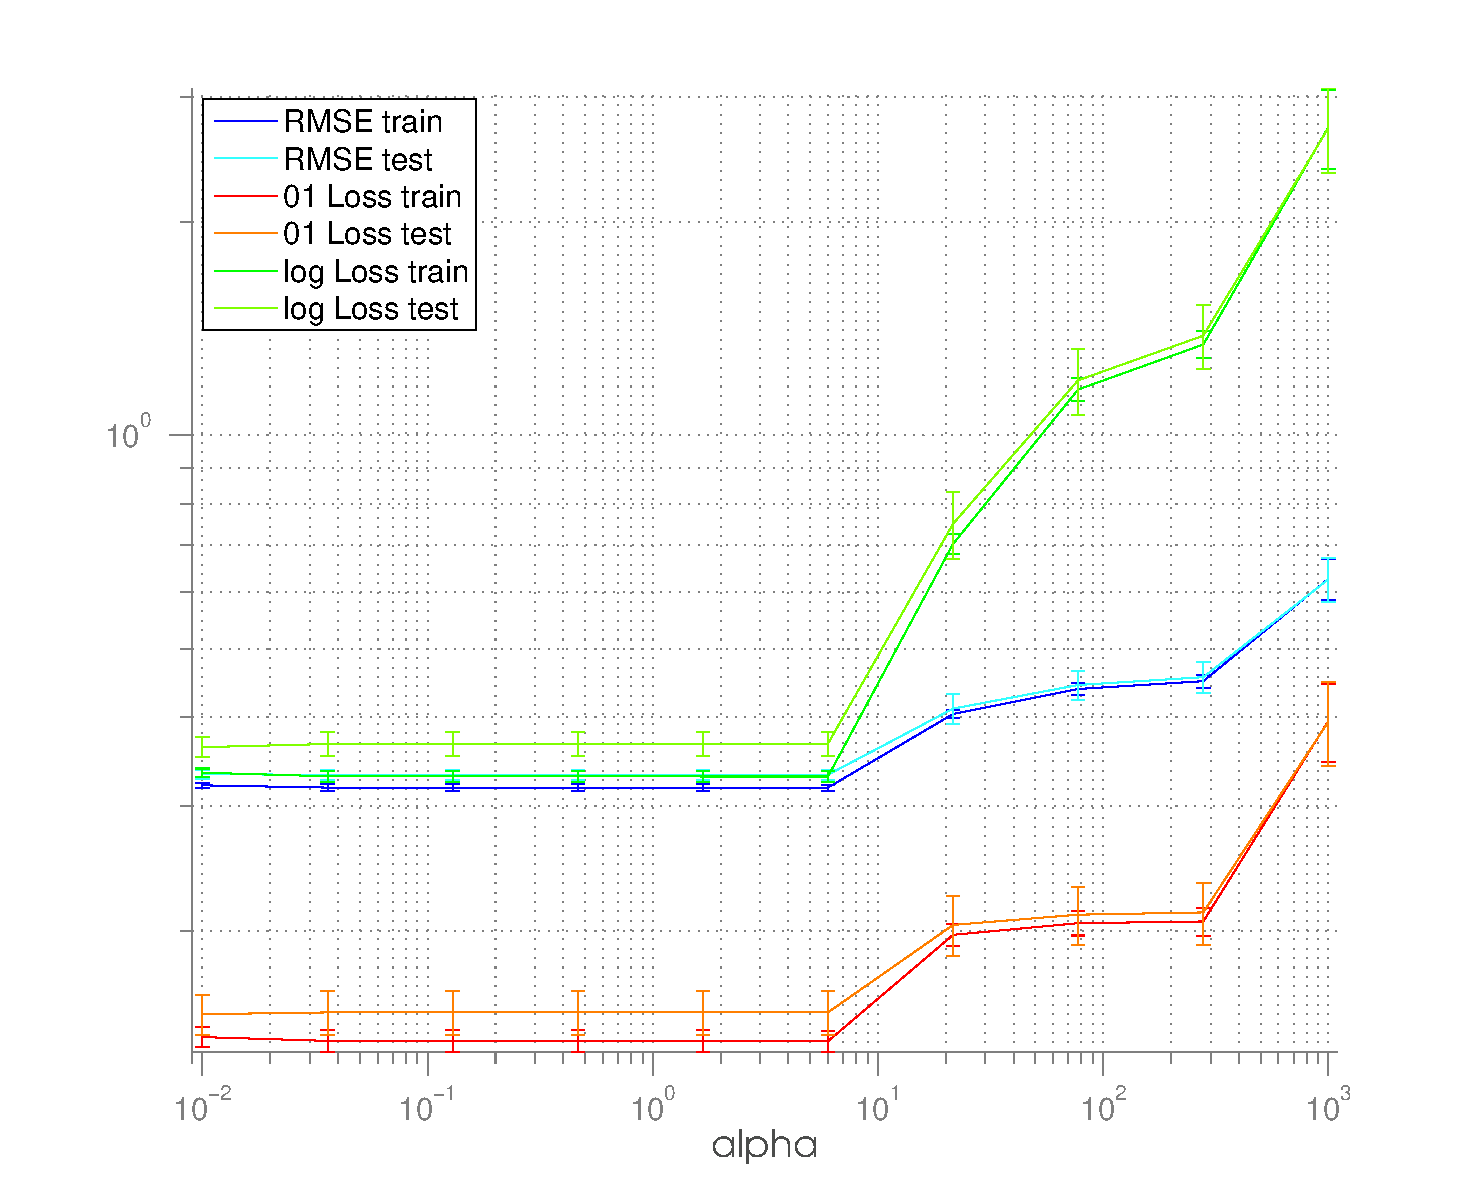
\includegraphics[width=2.5in]{figures/alphaLog.pdf} \label{fig:errors}}
\hfill
\subfigure[Evolution of RMSE when removing $\mathbf{x_{i}}$]{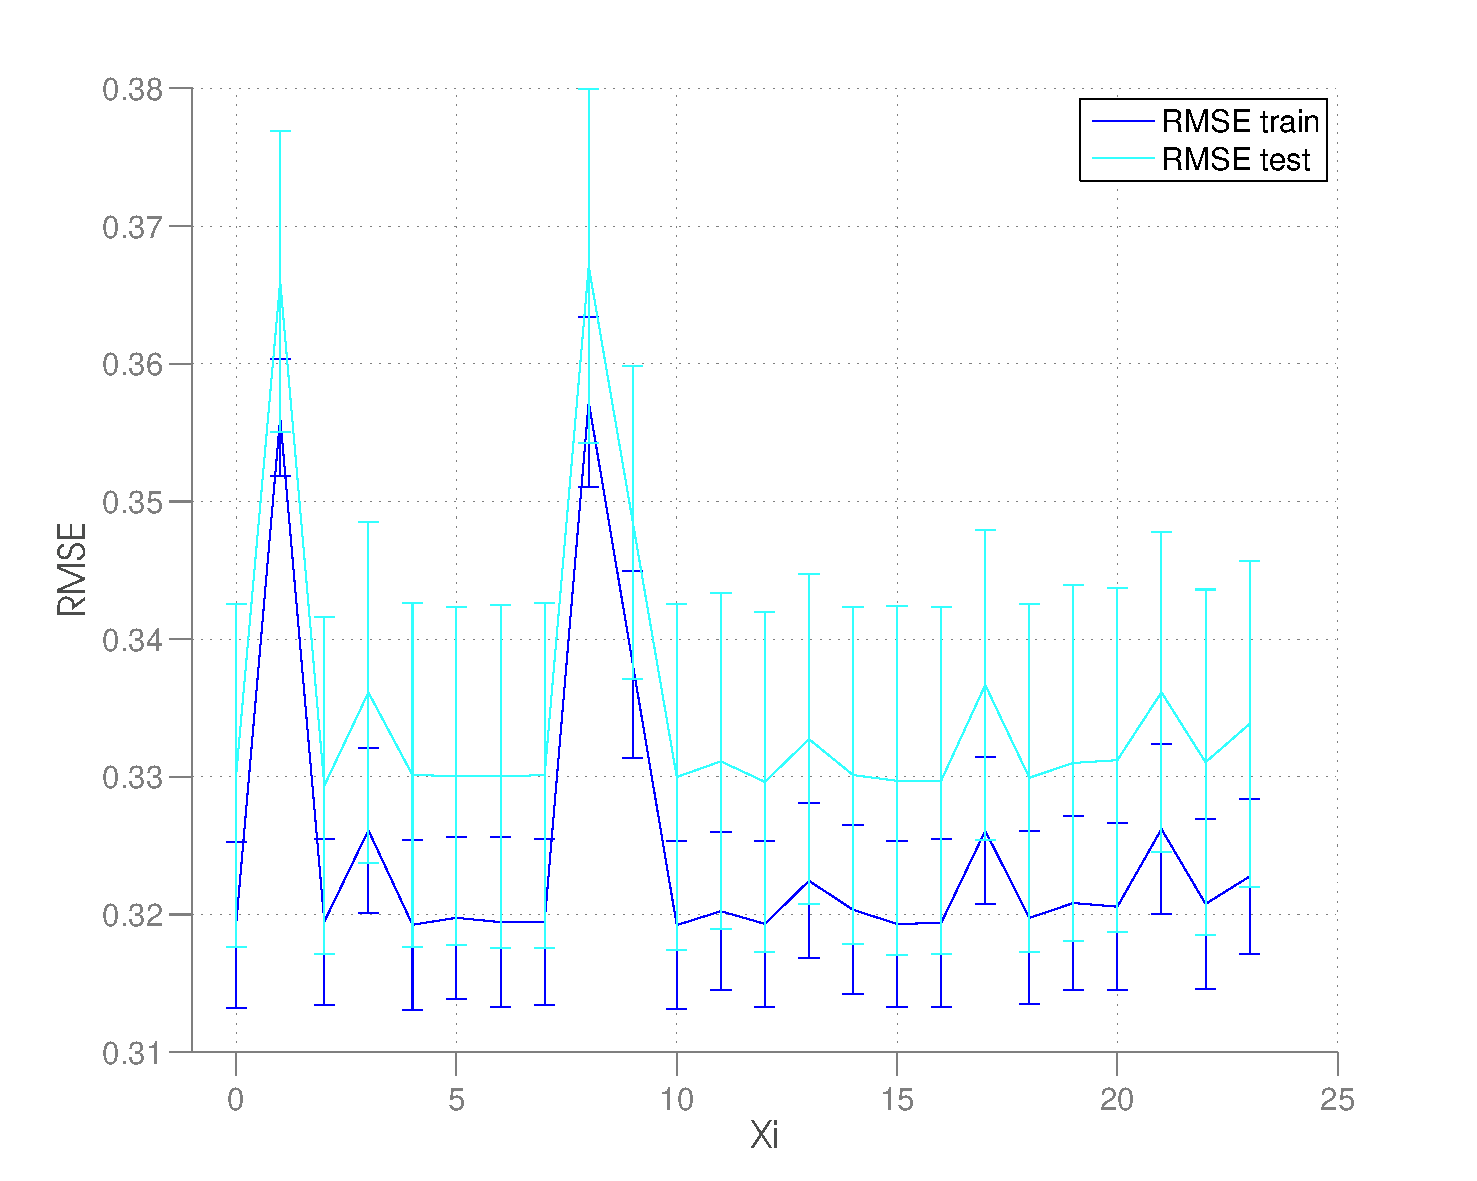
\includegraphics[width=2.5in]{figures/dimRedLR.pdf} \label{fig:dimRefLR}}

\subfigure[Evolution of RMSE when testing all interaction effects $\mathbf{x_{i} \cdot x_{j}}$.]{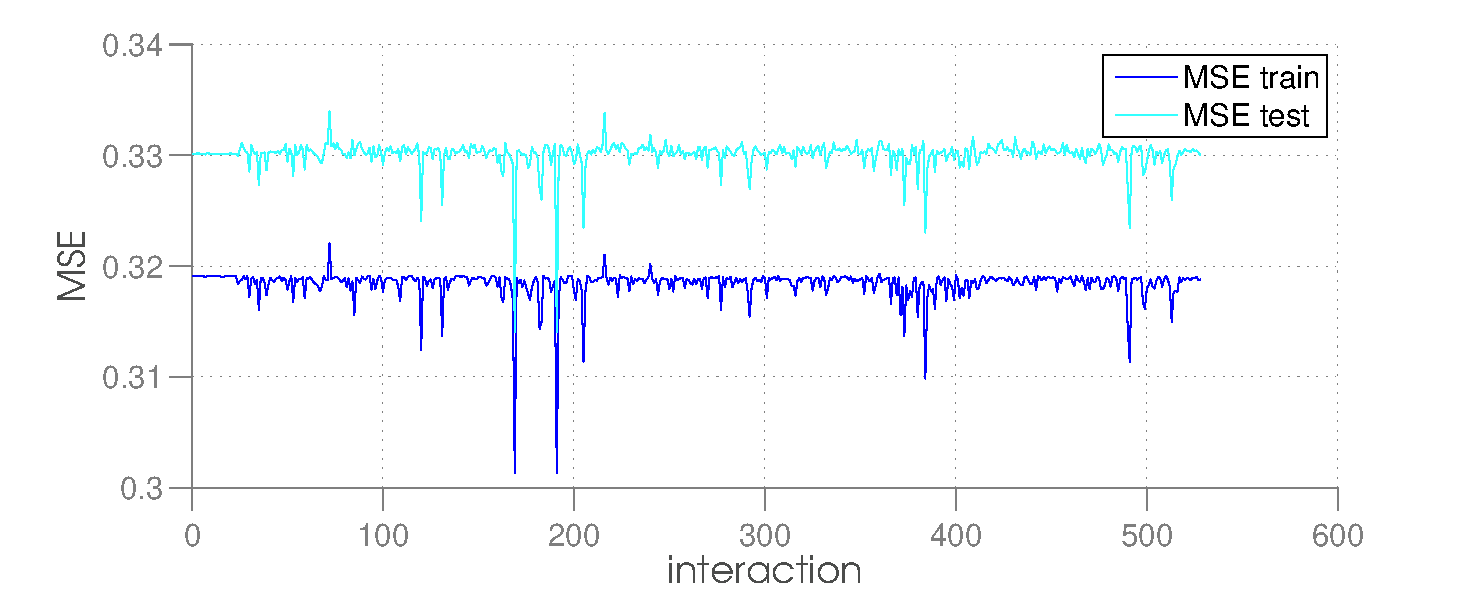
\includegraphics[width=2.5in]{figures/interaction.pdf} \label{fig:interaction}}
\hfill
\subfigure[Evolution of errors after adding the \textit{n} best interaction features.]{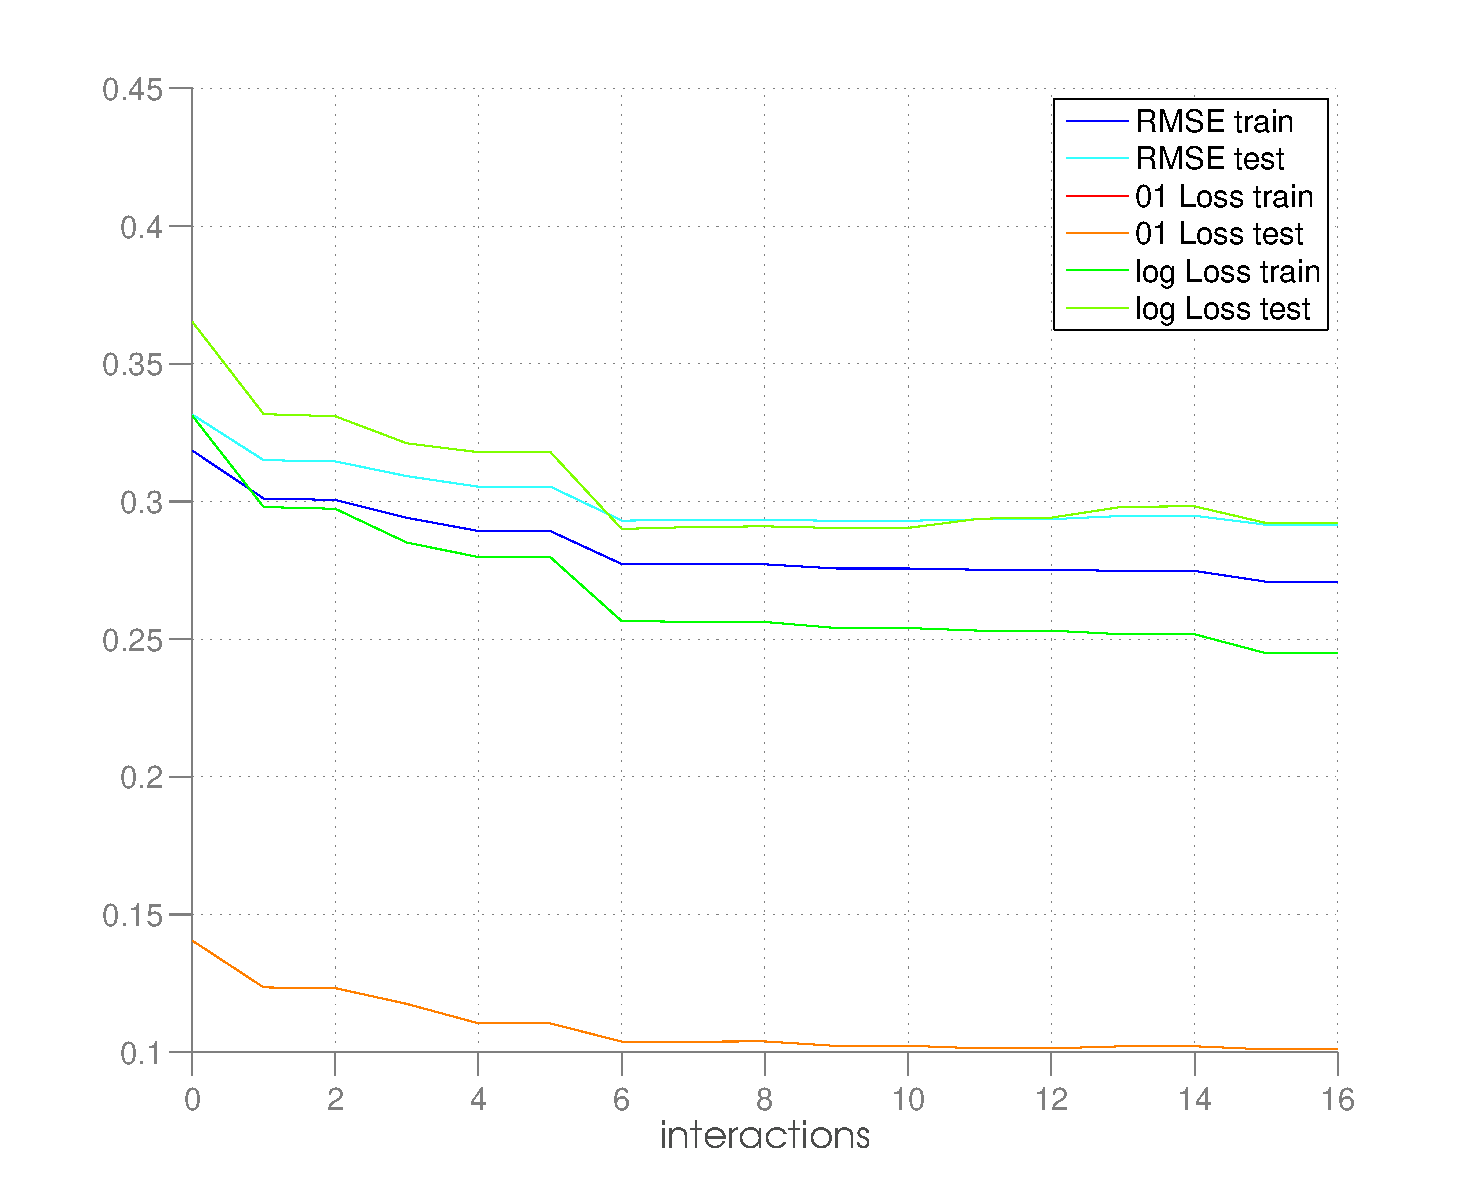
\includegraphics[width=2.5in]{figures/interactions3.pdf} \label{fig:interaction3}}

\caption{Analysis of data and settings}

\end{figure}


\subsection{Summary}

In this project, we were able to explore a complete dataset without any information about it beforehand. We developed methods to efficiently test our results and be confident about our predictions for regression and classification. We improved our test errors and predictions by applying transformations and adding interaction effects in our set of features, giving us satisfying results. 


\end{document}
